\section{Implementation and Evaluation}
We describe in detail our implementation method and evaluation procedure for answering 
our goals using the patent dataset.

\subsection{Analysis Methodology}

\begin{itemize}
\squish
\item Gephi and / or IGraph: Graph analysis and metric calculation~\cite{gephi, igraph}.

\item GraphViz, Gnuplot: Data visualization and result plotting~\cite{graphviz, gnuplot}.

\item Standard libraries and custom Python Scripts: For data extraction~\cite{python}.
\end{itemize}

\subsection{Experimental Setup}
The configuration of our experimental desktop machine is RAM $32$ GB, processor $XX.X$ GHz Intel i7 
and platform is Ubuntu $14.04$

\subsection{Graph Details}
Table~\ref{tab:model} gives the details about Graph G1 in
terms of its total number of nodes , edges , patents, the source node  of the graph
and the average distance between the source node and all other nodes .  
 We choose Thomas Edison as our source node
as he is one of the top and popular inventors in the patent dataset with maximum number of patents.
We calculate the shortest path of all other nodes from Thomas Edison. 
We run three algorithms particularly Djikstra shortest path algorithm, Bellman-ford and Johnson 
available in IGraph tool on our Graph G1. We observe that the average distance is $xx$ in our graph
from the source node.

\subsection{Results}
Table~\ref{tab:algos} shows the execution time for each of the three shortest path algorithms 
when run on our graph G1. We observe that Djikstra's algorithm takes $xx$ seconds, Bellman-ford takes
$xx$ seconds and Johnson algorithm takes $xx$ seconds to run on our experimental setup.
Figure~\ref{fig:distance} shows the result for the total number of inventors having the same
distance from Edison. This graph follows a normal distribution. Figure~\ref{fig:patent} shows the log-log graph of the total no.of patents
to total no.of inventors. We wil analyse whether this graph follows the power law distribution in our 
final analysis step. Figure~\ref{fig:distance_patent} shows the relation of the distance from Edison and
the no. of patents for an inventor. This graph also follows a normal distribution.



\begin{table*}[h] 
  %\centering
  \begin{tabular}{@{}c@{}} 
  \begin{minipage}{0.4\linewidth}
		\begin{center}
	  		\begin{tabular}{| l | l |}
				\hline
				{Type} & {Count} \\
				\hline
				\hline
				Inventors (Nodes) & 0.96 \\
				Co-authorships (Edges) & 1.29 \\
				Patents & 123123 \\
				Source Node & Thomas Edison\\
				Avg. Distance & 1.33 \\
				\hline
			\end{tabular}		
			\caption {Details of the co-authorship graph}
			\label{tab:model}

			\vspace{0.85cm}

			\begin{tabular}{| l | l |}
				\hline
				{Algorithm} & {Time} \\
				\hline
				\hline
				Algo I & 0.96 \\
				Algo II & 1.29 \\
				Algo III & 1.33 \\
				\hline
			\end{tabular}
			\caption {Performance of the three shortest path algorithms}
			\label{tab:algos}
		\end{center}

  \end{minipage}
  \hspace{0.05\linewidth}
  \begin{minipage}{0.45\linewidth}
      \begin{figure}[H]
          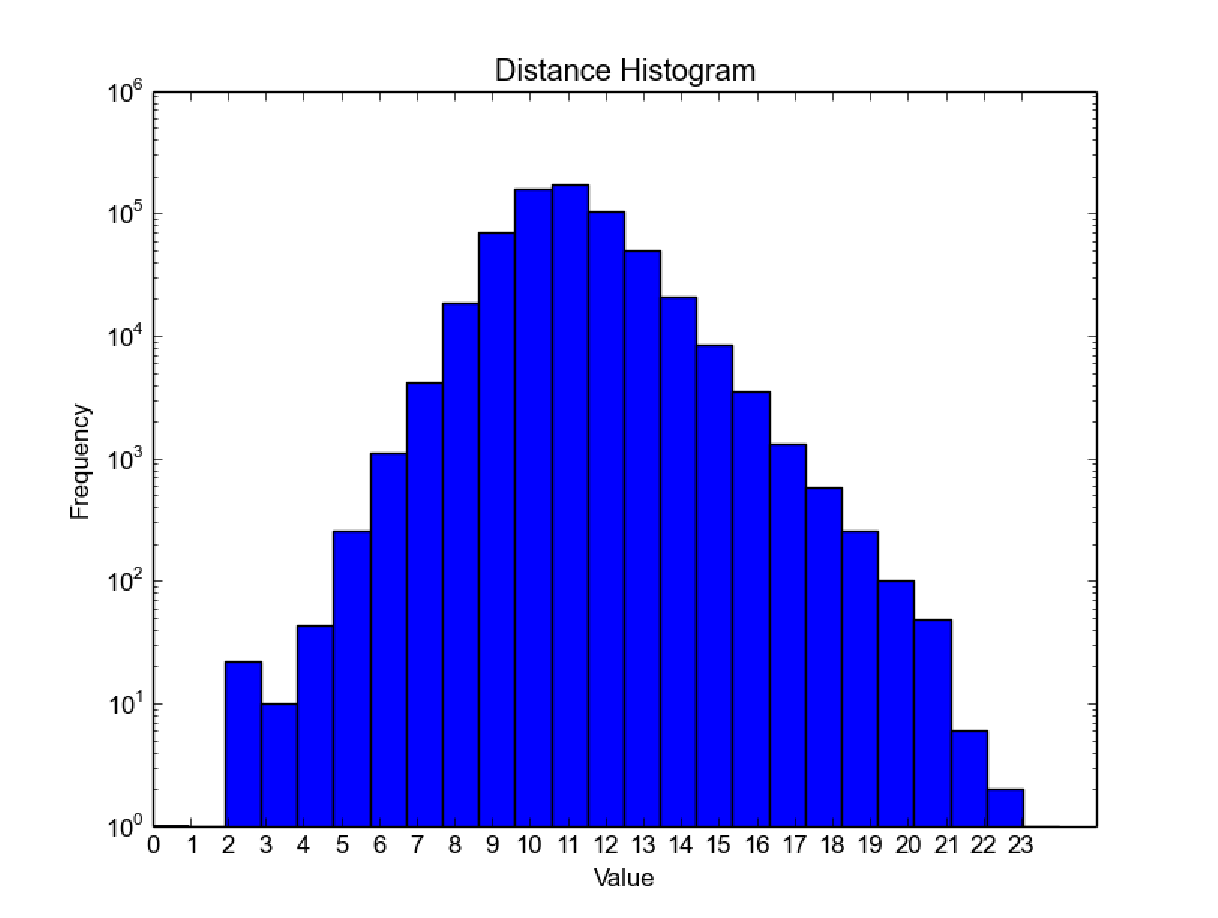
\includegraphics[scale=0.425]{../figures/distance.pdf}
          \caption{Graph shows the frequency of nodes on Y-axis and the distance from
		Edison on X-axis }
	  \label{fig:distance}
      \end{figure}
  \end{minipage}
  \end{tabular}
\end{table*}

% \end{minipage}

\begin{table*}[h] 
  %\centering
  \begin{tabular}{@{}c@{}} 
   \begin{minipage}{0.45\linewidth}
      \begin{figure}[H]
          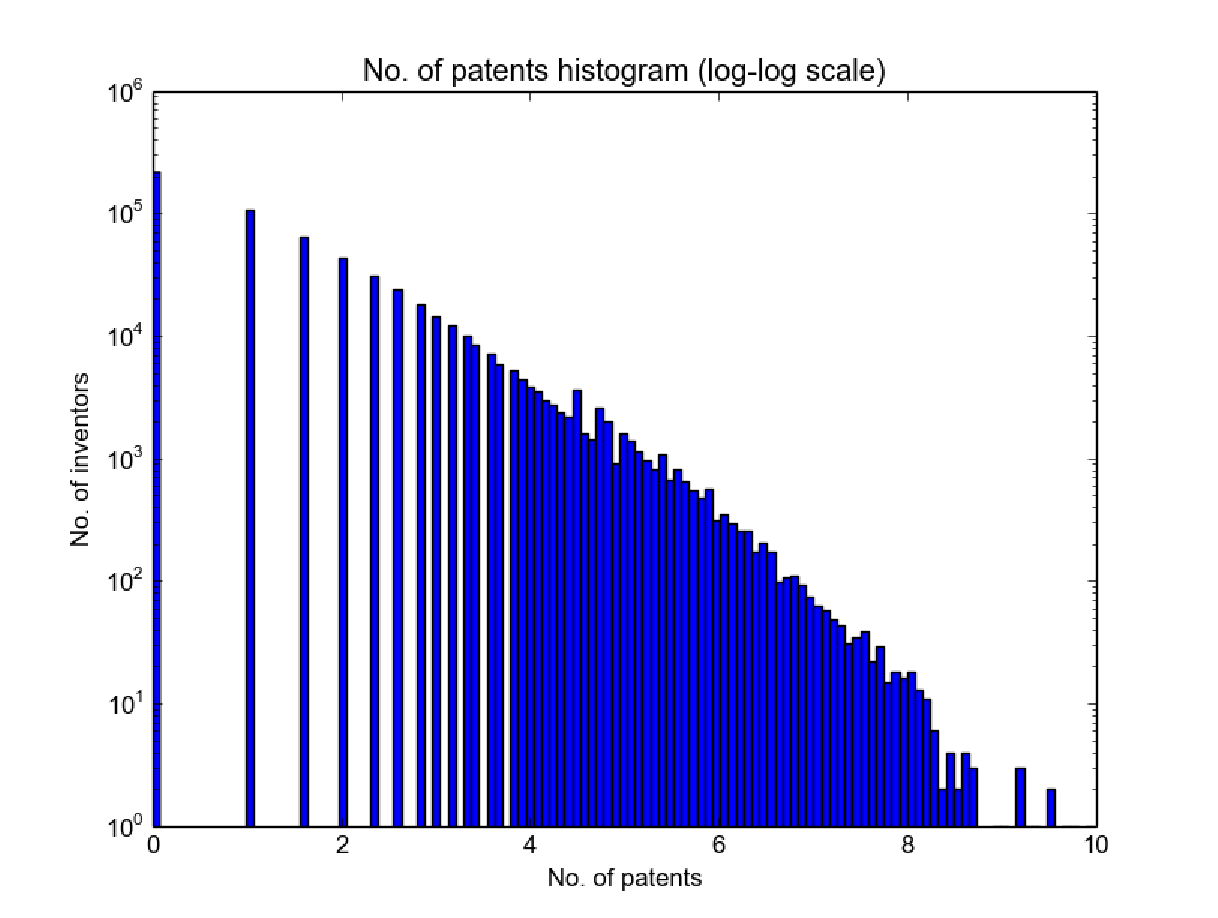
\includegraphics[scale=0.425]{../figures/patent.pdf}
          \caption{Log-log scale graph of no. of patents on Y-axis and the no.of inventors on X-axis}
	  \label{fig:patent}	
      \end{figure}
  \end{minipage}
  \begin{minipage}{0.45\linewidth}
      \begin{figure}[H]
          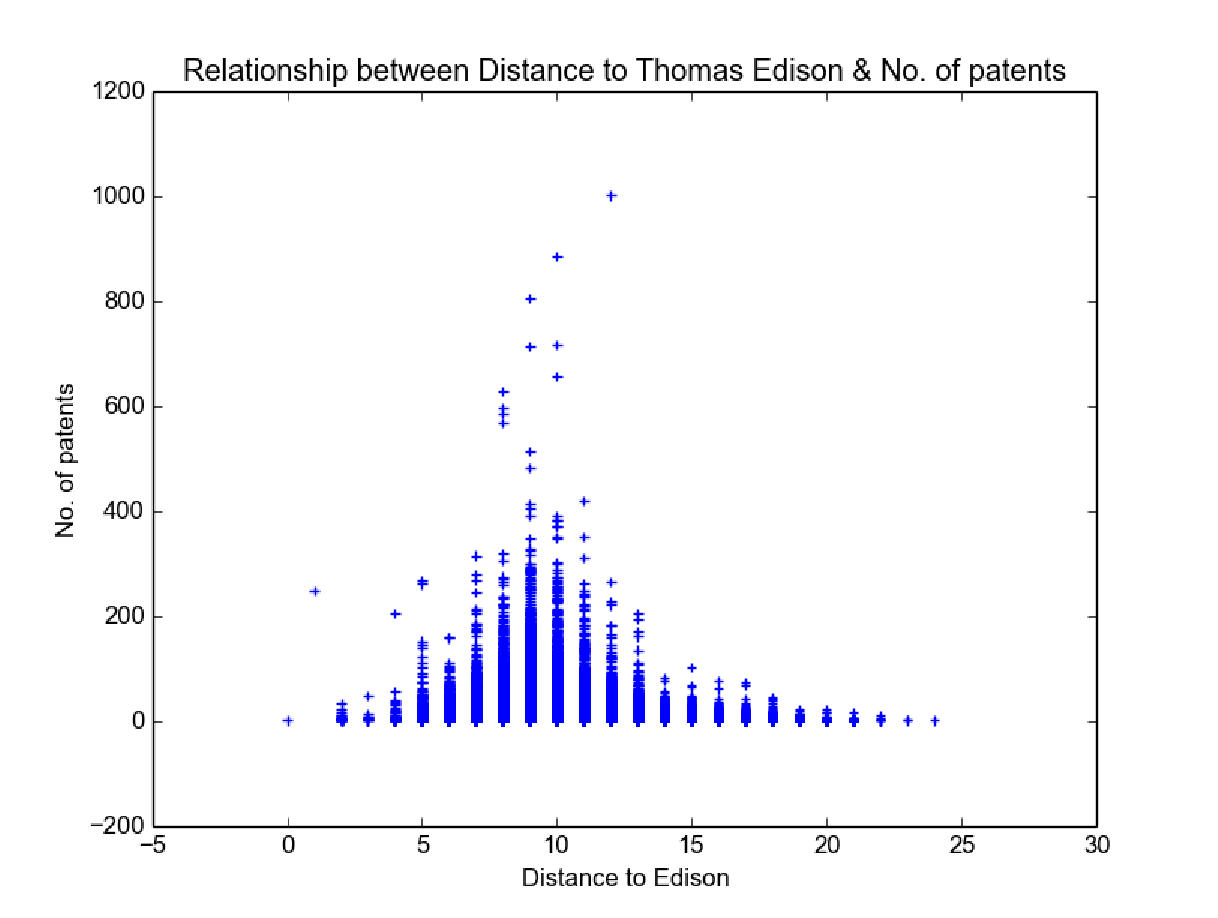
\includegraphics[scale=0.425]{../figures/distance_patent.pdf}
          \caption{Relationship graph of no. of patents of an inventor and his distance from Edison}
	  \label{fig:distance_patent}
      \end{figure}
  \end{minipage}
  \end{tabular}
\end{table*}


	\begin{itemize}
	\squish
		\item Ranking of organization according to the impact w.r.t to approved patents
		\item Plot of invention impact vs collaborative distance to answer Question 1
		\item Plot of invention impact vs organization to answer Question 2
		\item Plot of collaborative distance vs organization to answer Question 3
	\end{itemize}
